\section{Systeemoverzicht}

\begin{figure}[H]
	\centering
	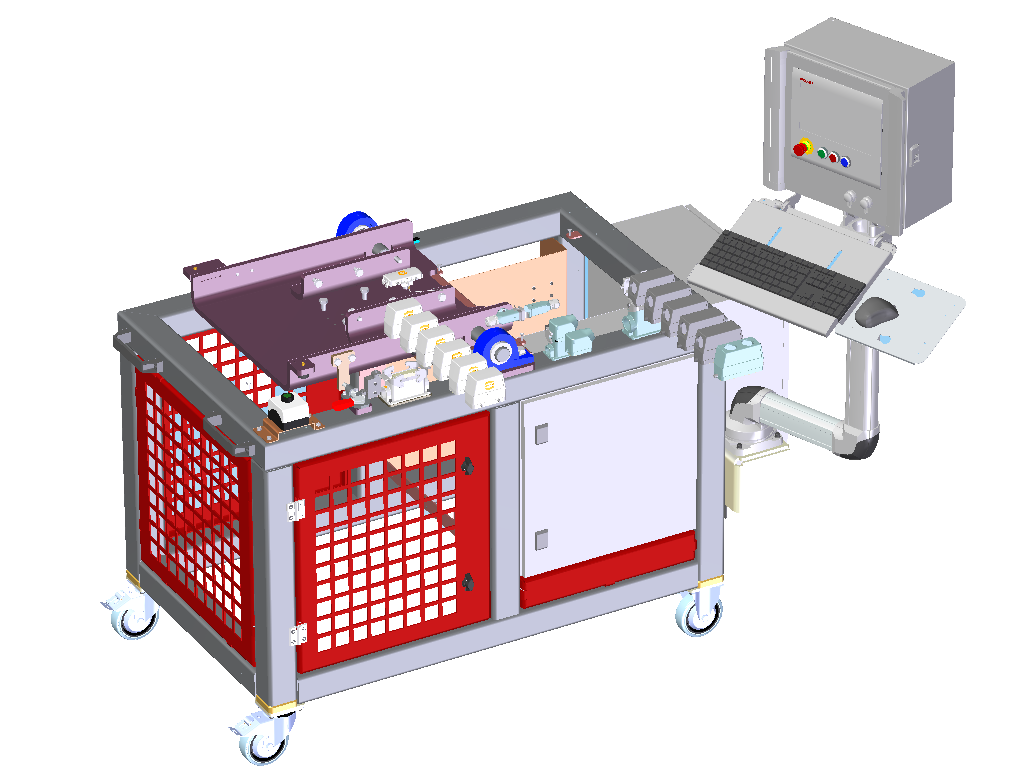
\includegraphics[width=\linewidth]{TestkastDrawing}
	\label{fig:TestkastDrawing}
	\caption{Testkast 3D tekening}
\end{figure}

In figuur \ref{fig:TestkastDrawing} is een afbeelding te zien van de huidige testkast. Mechanisch zal er in principe weinig veranderen aan de testkast behalve dat er een aantal gaten bij zouden kunnen komen voor spindels die nog niet gemonteerd kunnen worden op de testkast.

\vspace{0.5cm}

Er bevinden zich drie electrical boxen op de testkast deze zijn te zien in figuur \ref{fig:Foto3DModel3}.

\begin{itemize}
	\item \textbf{A} Deze box bevat de \gls{IPC} en knoppen zoals de stopknop, noodstop en de resetknop dit wordt ook wel het control panel genoemd.
	\item \textbf{B} Deze box heeft de \gls{AX5140} motordrive die is aangesloten op de \gls{IPC} via \gls{EtherCAT}. Daarnaast bevat deze box alle zekeringen, een hoofdschakelaar en powersupplies voor de testkast. Ook zitten er knoppen op box B om de LINAK actuator te laten bewegen deze wordt aangestuurd door een relais die op deze knoppen zit.
	\item \textbf{C} Deze box heeft alle \gls{IO} en een veiligheids \gls{PLC} die onafhankelijk van de \gls{IPC} functioneert. Deze \gls{IO} zijn aangesloten op de \gls{IPC} van box A via een EK1100 over \gls{EtherCAT}. Zodat de \gls{IPC} de \gls{IO} modules kan aansturen. 
\end{itemize}

\begin{figure}[H]
	\centering
	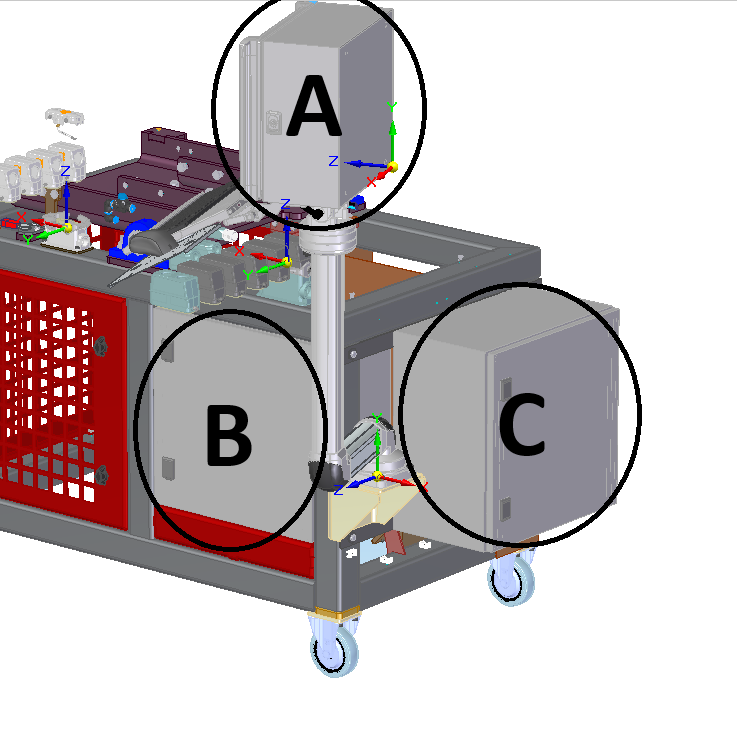
\includegraphics[width=\linewidth]{Foto3DModel3}
	\label{fig:Foto3DModel3}
	\caption{Testkast 3D tekening electrische kasten}
\end{figure}

Naast deze boxen zijn er nog een aantal componenten op de testkast zoals te zien in figuur \ref{fig:LINAK}.

\begin{itemize}
	\item \textbf{D} Dit is de LINAK actuator waarmee de montage plaat omhoog en omlaag bewogen kan worden. Deze LINAK wordt bestuurd door 2 knoppen op box B.
	\item \textbf{E} Dit is een lucht klep waarmee de toolchanger op spindels geopened of gesloten kan worden. De lucht klep wordt aangestuurd door een digitale uitgang in box C.
	\item \textbf{F} Dit is een deur schakelaar. Wanneer de deur geopened wordt mag de spindel voor de veiligheid niet meer draaien. Deze deur schakelaars zijn aangesloten op een veilige digitale input.
\end{itemize}

\begin{figure}[H]
	\centering
	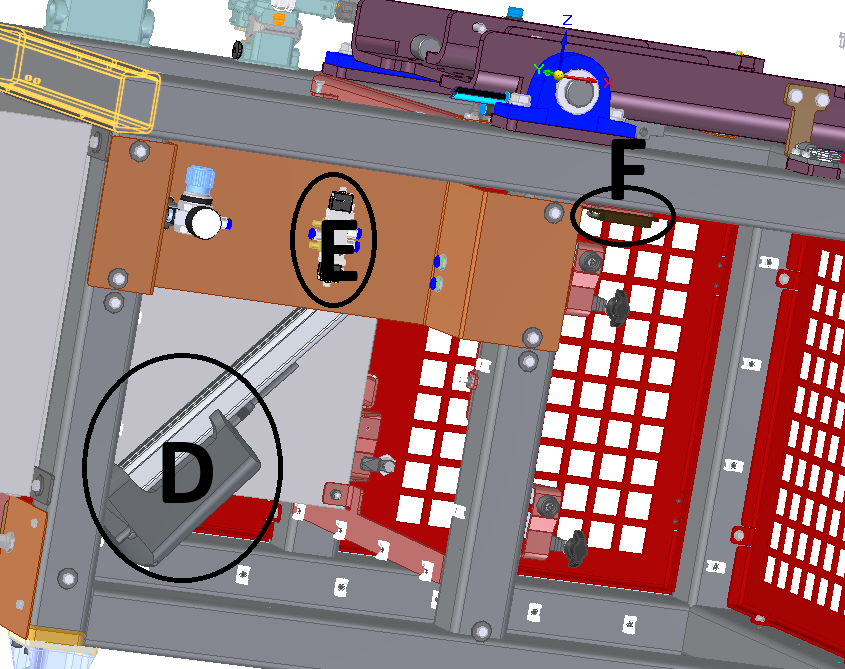
\includegraphics[width=\linewidth]{LINAK}
	\label{fig:LINAK}
	\caption{Testkast componenten}
\end{figure}

\begin{figure}[H]
	\centering
	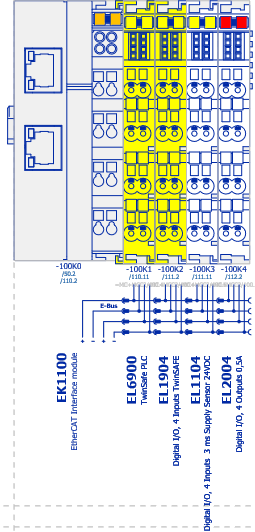
\includegraphics[width=0.7\linewidth]{IOTerminals}
	\label{fig:IOTerminals}
	\caption{IO Terminals in kast C}
\end{figure}